\documentclass{article}

% Language setting
% Replace `english' with e.g. `spanish' to change the document language
\usepackage[french]{babel}

% Set page size and margins
% Replace `letterpaper' with `a4paper' for UK/EU standard size
\usepackage[a4paper,top=2cm,bottom=2cm,left=3cm,right=3cm,marginparwidth=1.75cm]{geometry}

% Useful packages
\usepackage{amsmath}
\usepackage{graphicx}
\usepackage[colorlinks=true, allcolors=blue]{hyperref}

\title{Projet d'IMA201 : Palette automatique de couleur}
\author{Manon Heffernan, Cécile Tillerot}

\begin{document}
\maketitle

\begin{abstract}
Dans ce projet, nous avons implémenté la méthode de l'article "Automatic Color Palette" de J. Delon, A. Desolneux, J. L. Lisani and A. B. Petro, permettant de trouver une palette de quelques couleurs à partir d'une image.
\end{abstract}

\section{Quelques méthodes qui sont jugées inefficaces par l'article}

Nous avons commencé par tester deux méthodes qui donnent une représentation non-satisfaisante des couleurs dans une image : la méthode de median-cut, et la méthode k-means.\\

\subsection{Median-cut}

La méthode de median-cut consiste à diviser les intervalles en deux, à la médiane, et donc chercher une palette de couleurs où chacune représente un groupe de même proportion. Cependant, les petits détails colorés ressortent souvent de la même couleur que le fond, car leur couleur est vite minoritaire devant un fond uniforme. Nous avions fait un test avec l'image {\it ladybug}, et 64 couleurs ne suffisaient pas pour retrouver le rouge de l'insecte (Figure 1).\\

\begin{figure}[h]
    \centering
     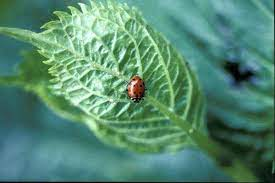
\includegraphics[width=5cm]{ladybug_example.jpeg}
     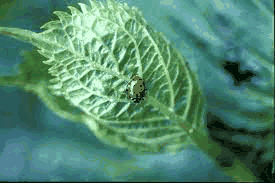
\includegraphics[width=5cm]{ladybug_2^16.jpg}
     \caption{Image originale et image après median-cut (k = 6)}
\end{figure}

\subsection{K-means}

Nous avons aussi implémenté l'algorithme de k-means, une technique populaire mais toujours pas satisfaisante pour notre but. Cette technique de clustering regroupe les points qui sont fortement concentrés autour d'une valeur (cluster). Cependant, elle dépend beaucoup de la position des germes et donne souvent des couleurs assez fades quand l'arrière-plan est sombre. C'est cette technique que l'on cherche à améliorer en déterminant des germes judicieux.\\

En Figure 2, on a l'image {\it bouquet} sur un fond noir, et le résultat de l'algorithme k-means.\\

\begin{figure}[h]
    \centering
     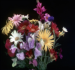
\includegraphics[width=5cm]{bouquet.pdf}
     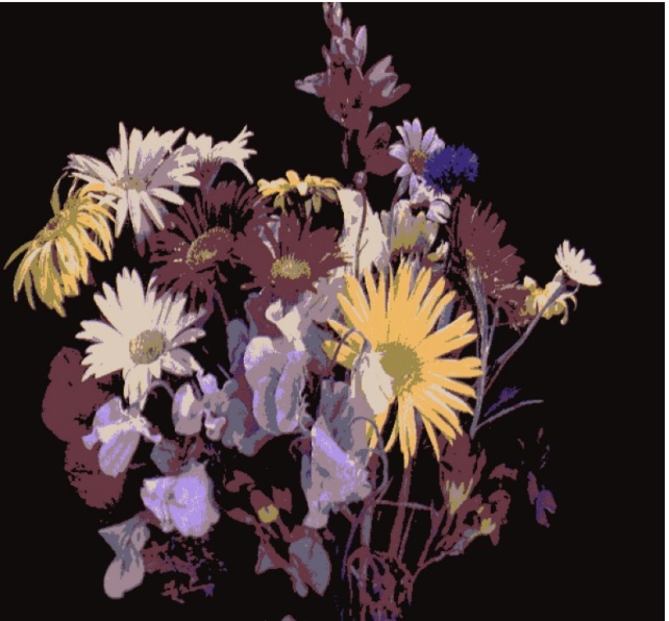
\includegraphics[width=5cm]{bouquet_kmeans.pdf}
     \caption{Image originale et image après k-means (k = 30)}
\end{figure}

Ces deux algorithmes sont paramétriques, et ils ne donnent pas des résultats satisfaisants. L'article que nous avons lu nous a permis de remédier à ces problèmes.\\

\section{Algorithme de l'APoCa}

\subsection{L'espace de couleur choisi}

Manon explique le hsi...

Pour notre implémentation, nous sommes obligées de faire une représentation "HSI modifiée", qui comporte les trois composantes H, S et I du pixel, mais aussi les classes dans lesquelles est le pixel pour chaque composante, en fonction des segmentations obtenues.

\subsection{Segmentations et quantifications nécessaires}

L'algorithme ACoPa repose sur la bonne segmentation des histogrammes des dimensions H,S et I. Pour cela, nous avons choisi de faire une fonction différente par dimension. On calcule d'abord la segmentation sur H, ce qui nous donne des groupes de pixels avec plus ou moins la même couleur. Puis on fait la segmentation des histogrammes selon S de chaque groupe de pixels. Enfin, sur chaque sous-groupe, on fait une segmentation selon I.\\

On définit pour chaque segmentation une constante  Q$\_$hue,  Q$\_$sat et Q$\_$int qui donnent la quantification des composantes H, S, I. Comme nous sommes passés dans l'espace HSI avec des formules mathématique, les grandeurs ne sont pas entières et limitées entre 0 et 255 (comme en RGB), et il faut donc quantifier pour ne pas avoir un histogramme avec une distribution uniforme (1 valeur, 1 pixel), et diminuer le temps de calcul. On voit par exemple sur la figure 3 pour l'image {\it teletubbies} comment différentes valeurs de Q$\_$hue,  Q$\_$sat et Q$\_$int peuvent influencer les résultats de l'algorithme APoCa, surtout si l'on considère la condition du grey cylinder, qui peut exclure complètement certaines teintes de l'image si la saturation est faible et que Q$\_$hue est élevé. Ici, le jaune et le violet sont remplacés par du vert et du rouge, car les pixels de ces teintes n'étaient pas suffisamment saturées.\\

\begin{figure}[h]
    \centering
    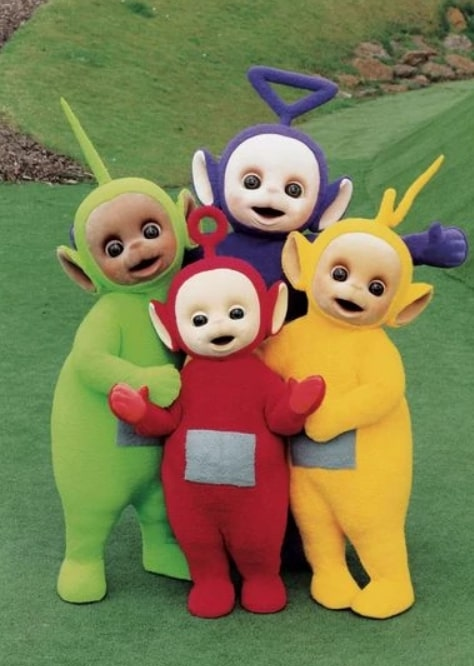
\includegraphics[width=3cm]{teletubbies.jpg}
    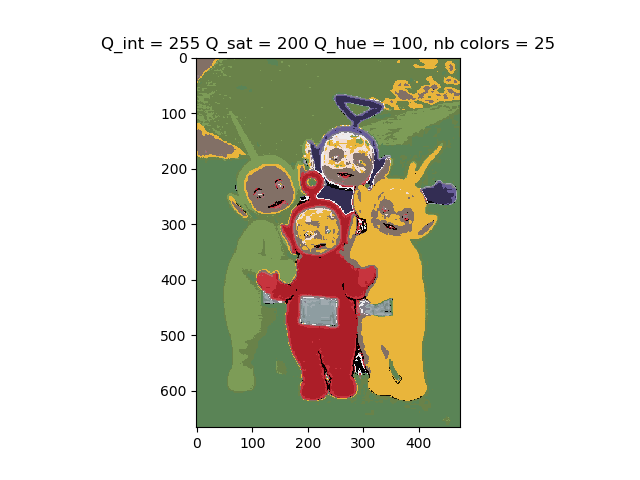
\includegraphics[width=5.5cm]{fig3_milieu.png}
    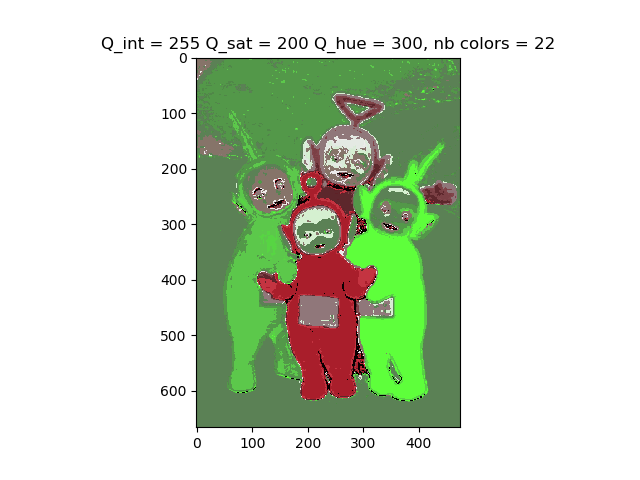
\includegraphics[width=5.5cm]{fig3_droite.png}
    \caption{Images de télétubbies : à gauche, originale ; au milieu, avec Q$\_$hue = 100 après FTC ; à droite, avec Q$\_$hue = 300 après APoCa}
\end{figure}

Cette segmentation nous permet aussi d'éliminer certaines valeurs de la composante H, définies dans le papier comme un {\it grey cylinder}. La valeur de saturation pour ces pixels est si faible qu'ils apparaissent tous plus ou moins gris, et le papier recommande de ne pas les prendre en compte dans la segmentation de H. On les rajoute cependant dans le calcul des autres segmentations, en les rattachant au groupe de teintes auquel ils appartiennent, sans les avoir pris en compte pour calculer ces groupes. Voici l'effet de cette limitation sur une image avec des couleurs peu saturée, en figure 4. Appliquer cette condition peut permettre aux couleurs uniformes et peu saturées de l'arrière-plan d'être moins présentes, et de laisser de la place aux couleurs plus vives et saturées du premier plan (la peau de la jeune femme par exemple). La différence est subtile, mais notable dès l'étape de l'APoCa.\\

\begin{figure}[h]
    \centering
    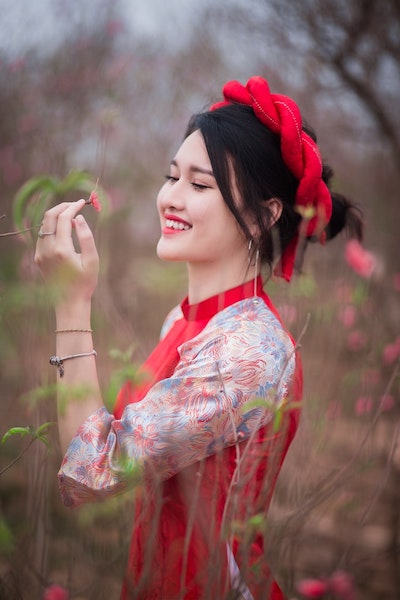
\includegraphics[width=2.7cm]{girl.jpeg}
    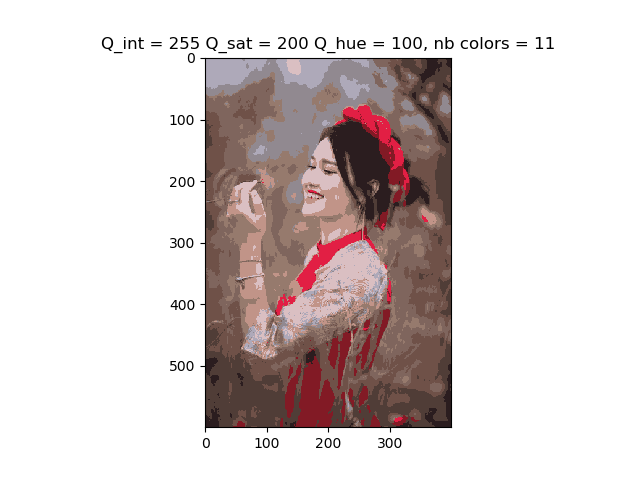
\includegraphics[width=6cm]{fig4_gauche.png}
    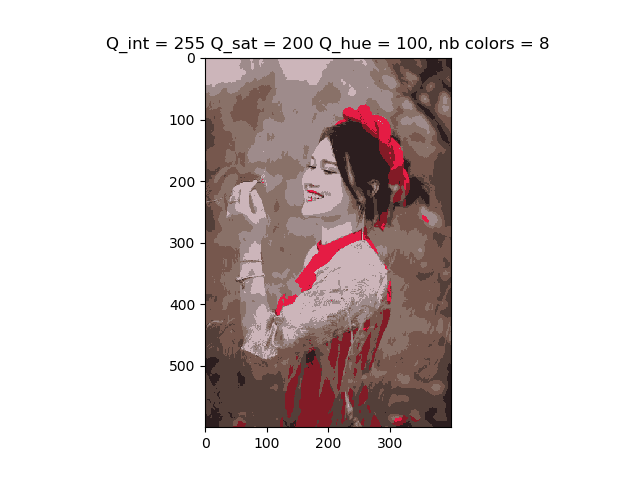
\includegraphics[width=6cm]{fig4_droite.png}
    \caption{Influence du grey cylinder : à gauche, l'original ; au milieu, avec une condition que S soit supérieur à Q$\_$hue+20/2$\pi$ ; à droite, sans condition sur le grey cylinder}
\end{figure}

\subsection{Le principe de l'algorithme de FTC}

Il faut appliquer cet algorithme sur l'histogramme de chaque dimension.\\ 

L'agorithme de segmentation "Fine To Coarse" (FTC) permet de diviser un histogramme en plusieurs groupes de pixels tel qu'il est acceptable de dire que chaque groupe suive une loi unimodale. On part d'une segmentation "fine" (une liste des minima locaux), puis on essaie de regrouper deux segments adjacents en regardant si l'histogramme se rapproche de son estimateur de Grenander (qui lui est unimodal).\\

Nous devons envisager tous les cas possibles pour regrouper les segments, et calculons donc deux estimateurs : un croissant pour le côté gauche du maximum, et un décroissant pour le côté droit du maximum. L'estimateur de Grenander transforme un histogramme non monotone en histogramme croissant (ou décroissant).  Nous avons utilisé l'algorithme des Pool Adjacents Violators pour le construire : pour l'estimateur croissant par exemple, on parcourt le segment et si on arrive à un point qui est inférieur au précédent, on le met au même niveau, et de même jusqu'au prochain point qui continue à augmenter. Cet estimateur est notre distribution théorique (croissante ou décroissante), et le test statistique détermine si l'estimateur n'est pas aberrant, c'est-à-dire si l'histogramme peut être considéré croissant puis décroissant sur une partie, et donc si on peut regrouper les segments et continuer à essayer avec les segments alentours.\\

En figure 5, nous avons réalisé quelques tests d'implémentation de l'algorithme des Pool Adjacent Violators sur des histogrammes simples.\\

\begin{figure}[h]
    \centering
    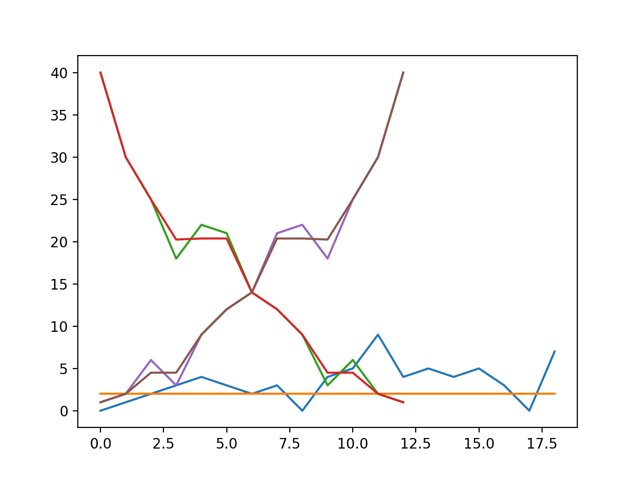
\includegraphics[width=9cm]{fig5.png}
    \caption{Des histogrammes (vert, violet, bleu) et leurs estimateurs de Grenander (rouge, marron, orange respectivement)}
\end{figure}

\subsection{Le test d'unimodalité}

On trouve que l'hypothèse d'unimodalité est vraie si le résultat du test statistique rapprochant l'estimateur de Grenander décrit dans la section suivante est 0. Il reste à choisir et implémenter ce test. Dans le papier, il est dit que la solution optimale est un test multiple, qui teste plus d'une hypothèse. Mais un test du khi-deux peut aussi convenir pour déterminer si un histogramme est la réalisation d'une loi. \\

Les hypothèses sont : \\

$H_0$ : L'histogramme peut être vu comme la réalisation de la loi que suit l'estimateur de Grenander.\\

$H_1$ : L'histogramme ne peut pas être vu comme la réalisation de la loi que suit l'estimateur de Grenander.\\

Et le test statistique :\\

$\delta(T) = 1$ si $T(X) \geq C $ avec $C = q_{\chi^{2}}(1-{\alpha})$ et $\delta(T) = 0$ sinon, 
où $q_{\chi2}$ est la fonction quantile de la loi ${\chi}^{2}(k)$, ${\alpha}$ choisi à 0.01, un niveau standard du test du khi-deux.\\

T est l'estimateur de la loi du khi-deux calculé à partir de l'histogramme et de l'estimateur de Grenander. Sa formule est :\\

$T = \sum \limits _{j=1} ^{len(histo)}\frac {(histo[j]-estimateur[j])^2}{estimateur[j]})$ \\

Avec ce test et les sections précédentes, nous avons tous les élements nécessaires pour implémenter l'algorithme de FTC, et pour déterminer une segmentation selon les principaux modes des histogrammes selon H, S et I.\\

\section{Détermination de la palette de couleurs}

\subsection{Calcul des couleurs représentatives, et images obtenues après l'algorithme de l'APoCa (sans k-means)}

En ayant segmenté les trois histogrammes selon H, S, et I, les uns dépendemment des autres, on sait classer les pixels dans un groupe de pixels qui est unimodal. Pour afficher une image et voir la palette de couleurs proposée avant k-means, il faut donc déterminer quelle valeur on donne aux pixels d'un même groupe (de H, de S ou de I). C'est le rôle de nos fonctions "compute mode", qui repèrent le maximum et qui choisit cette valeur pour représenter la classe.\\

Pour afficher l'image, on a plus qu'à associer à chaque pixel les valeurs sur H, S et I qu'il doit prendre selon sa classification. On obtient alors des images plus satisfaisantes que dans les méthodes précédentes, avec moins de couleurs. Par exemple, pour {\it ladybug} (voir chapitre 1), le rouge n'est plus perdu, tout en ayant seulement 10 couleurs sur l'image.\\

\begin{figure}[h]
    \centering
    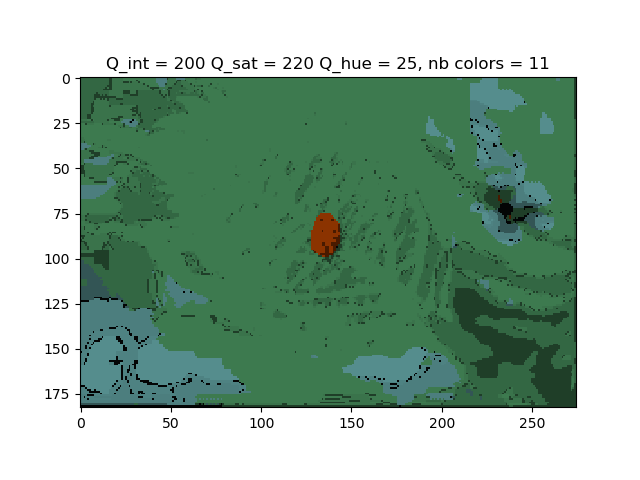
\includegraphics[width=10cm]{fig6.png}
    \caption{Résultat de la fonction apoca pour l'image {\it ladybug}}
\end{figure}

Cependant, une image avec des objets de couleurs assez proches peuvent se retrouver perturbées par l'opération : dans l'exemple de la figure 7, on ne distingue plus le plateau en bois de la surface de la table, ni des carottes qui ont la même couleur. Ceci peut poser problème pour reconnaître des objets, si les détails et les ombres ne sont pas représentées par une classe de pixels, et que les couleurs des objets sont assez similaires...\\

\begin{figure}[h]
    \centering
    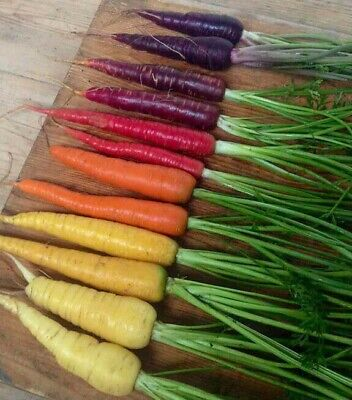
\includegraphics[width=4cm]{carottes.jpg}
    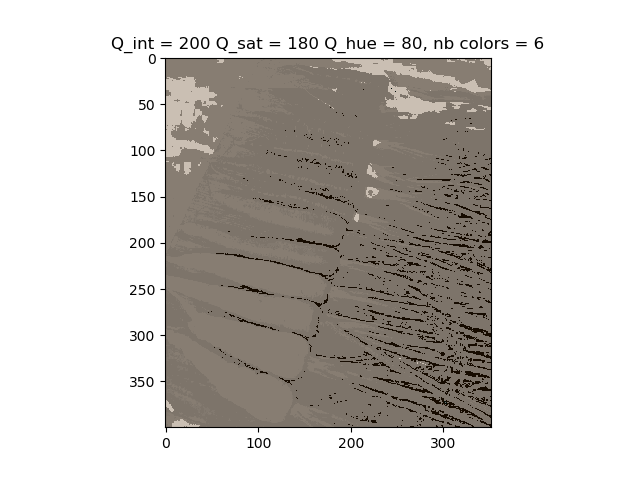
\includegraphics[width=7cm]{fig7.png}
    \caption{À droite, image {\it carottes} ; à gauche, résultat de la fonction apoca}
\end{figure}

L'algorithme de k-means, qui réajuste les centres en prenant en compte la forme des clusters autour d'un mode, est donc nécessaire pour terminer le calcul de notre palette de couleurs.\\

\subsection{Calcul des couleurs représentatives après k-means, et images obtenues à la fin}

Dans notre fonction apoca, nous avons enregistré les couleurs qui seront finalement représentées sur l'image, et leur nombre. On applique ensuite l'algorithme de k-means à l'image avec ces centres initiaux. En récupérant les nouveaux centres des clusters, on applique la fonction kmeans.predict pour retrouver dans quelle classe est finalement chaque pixel, et on lui affecte la valeur du centre de la classe.\\

Cette méthode retire le choix difficile du paramètre k et des centres de k-means, car tous deux sont déterminés de manière unique pour chaque image, en se basant sur son histogramme. Les résultats après k-means sont grandement améliorés, pour {\it carottes} et {\it ladybug} que nous avons vu plus haut par exemple. \\

\begin{figure}[h]
    \centering
    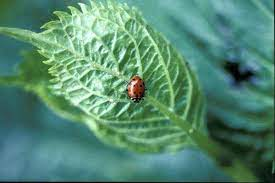
\includegraphics[width=5cm]{ladybug_example.jpeg}
    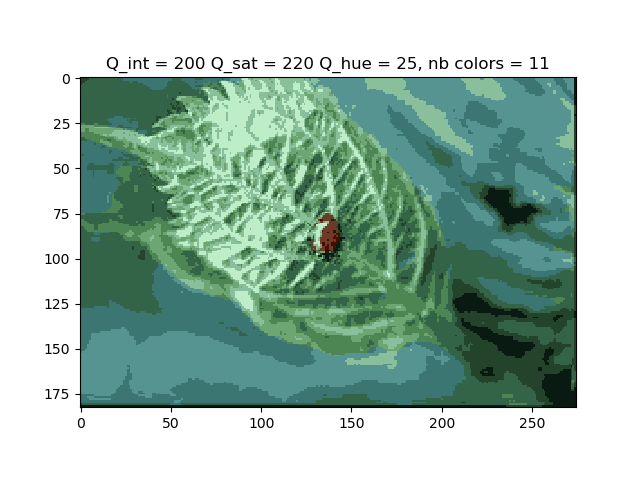
\includegraphics[width=6cm]{fig8.png}
    \caption{À gauche, image {\it ladybug} ; à droite, résultat final}
\end{figure}

\begin{figure}[h]
    \centering
    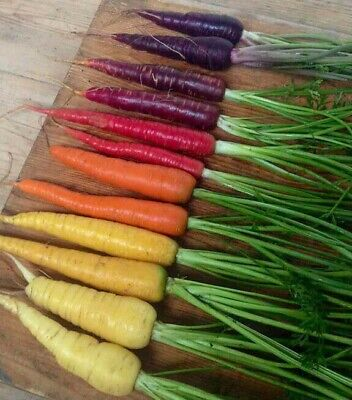
\includegraphics[width=4cm]{carottes.jpg}
    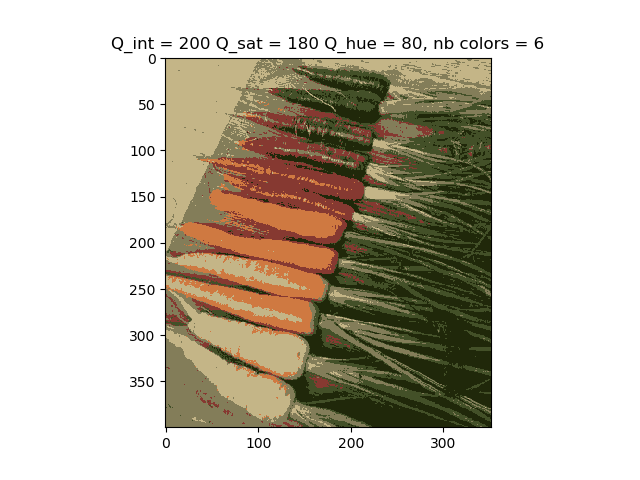
\includegraphics[width=7cm]{fig9.png}
    \caption{À gauche, image {\it carottes} ; à droite, résultat final}
\end{figure}

Nous devons cependant souvent ajuster nos paramètres de quantification en fonction des images, même si nous avons remarqué qu'une valeur de I autour de 255, de H en dessous de 100 et de S autour de 200 suffisaient dans la plupart des cas.\\

\subsection{Affichage graphique}

Méthode à implémenter pour les petits carrés...

\section{Test sur des images présentant des difficultés particulières}

- Low contrast\\
- Low luminosity\\
- Multicolore\\
- Dégradé -> favorisation d'une teinte ? d'une intensité ?\\
- On met une bibliographie ?


\end{document}